\begin{flushleft}
{\Huge Punschvisor\\}
\vspace{1cm}
\Large{
Punsch drickes antingen mycket kall till efterrätt alla dagar i veckan,
eller varm till torsdagens ärtsoppa. Det kan även hända att det
slinker ner en liten en till onsdags-hofflan. En gång i tiden hade
punschen systemets högsta apk - Alkohol per Krona - och många tror att
det är därför det alltid har druckits mycket punsch i studentikosa
sammanhang. Andra tror det beror på att det är gott.}
\end{flushleft}
\vspace{2cm}
\begin{center}
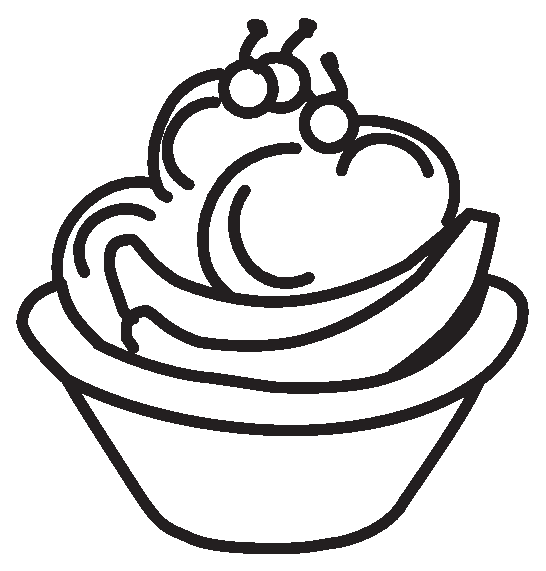
\includegraphics[width=5cm]{bilder/47.eps}
\end{center}
\newpage

\inputsong{gamlakall}

\inputsong{gamlavarm}

\newpage

\inputsong{punschvisaf}

\newpage


\inputsong{festu}

\inputsong{studiemedelsrondo}

\newpage

\inputsong{punschengul}

\inputsong{djungelpunsch}

\newpage

\inputsong{enkoppmedpunsch}

\newpage

\inputsong{gudarnaspunschvisa}

\inputsong{punschschottis}

\newpage

\inputsong{anglapunsch}

\newpage

\inputsong{punschlunch}

\inputsong{skogshogskolanspunschvisa}

\inputsong{jaggillar}

\newpage

\inputsong{arterochpunsch}

%\inputsong{narsompunschen}

\newpage
\inputsong{tvekaniforpunschen}

\newpage

\inputsong{punschpolkett}

\inputsong{minpunsch}

\newpage

\inputsong{punschpunsch}

\inputsong{punchpunch}

\newpage

\inputsong{vadjantillpunschen}

\inputsong{sistapunschvisan}






